\documentclass{beamer}

%\usepackage[table]{xcolor}
\mode<presentation> {
  \usetheme{Boadilla}
%  \usetheme{Pittsburgh}
%\usefonttheme[2]{sans}
\renewcommand{\familydefault}{cmss}
%\usepackage{lmodern}
%\usepackage[T1]{fontenc}
%\usepackage{palatino}
%\usepackage{cmbright}
  \setbeamercovered{transparent}
\useinnertheme{rectangles}
}
%\usepackage{normalem}{ulem}
%\usepackage{colortbl, textcomp}
\setbeamercolor{normal text}{fg=black}
\setbeamercolor{structure}{fg= black}
\definecolor{trial}{cmyk}{1,0,0, 0}
\definecolor{trial2}{cmyk}{0.00,0,1, 0}
\definecolor{darkgreen}{rgb}{0,.4, 0.1}
\usepackage{array}
\beamertemplatesolidbackgroundcolor{white}  \setbeamercolor{alerted
text}{fg=red}
\newtheorem{assumption}{Assumption}

\setbeamertemplate{caption}[numbered]\newcounter{mylastframe}

%\usepackage{color}
\usepackage{tikz}
\usetikzlibrary{arrows}
\usepackage{colortbl}
%\usepackage[usenames, dvipsnames]{color}
%\setbeamertemplate{caption}[numbered]\newcounter{mylastframe}c
%\newcolumntype{Y}{\columncolor[cmyk]{0, 0, 1, 0}\raggedright}
%\newcolumntype{C}{\columncolor[cmyk]{1, 0, 0, 0}\raggedright}
%\newcolumntype{G}{\columncolor[rgb]{0, 1, 0}\raggedright}
%\newcolumntype{R}{\columncolor[rgb]{1, 0, 0}\raggedright}

%\begin{beamerboxesrounded}[upper=uppercol,lower=lowercol,shadow=true]{Block}
%$A = B$.
%\end{beamerboxesrounded}}
\renewcommand{\familydefault}{cmss}
%\usepackage[all]{xy}

\usepackage{tikz}
\usepackage{lipsum}

 \newenvironment{changemargin}[3]{%
 \begin{list}{}{%
 \setlength{\topsep}{0pt}%
 \setlength{\leftmargin}{#1}%
 \setlength{\rightmargin}{#2}%
 \setlength{\topmargin}{#3}%
 \setlength{\listparindent}{\parindent}%
 \setlength{\itemindent}{\parindent}%
 \setlength{\parsep}{\parskip}%
 }%
\item[]}{\end{list}}
\usetikzlibrary{arrows}
%\usepackage{palatino}
%\usepackage{eulervm}
\usecolortheme{lily}

\newtheorem{com}{Comment}
\newtheorem{lem} {Lemma}
\newtheorem{prop}{Proposition}
\newtheorem{thm}{Theorem}
\newtheorem{defn}{Definition}
\newtheorem{cor}{Corollary}
\newtheorem{obs}{Observation}
 \numberwithin{equation}{section}

%Box Types


\title[Voter ID] % (optional, nur bei langen Titeln nötig)
{Obstacles To Estimating Voter ID Laws' Effect on Turnout}

\author{Justin Grimmer}
\institute[University of Chicago]{Associate Professor\\Department of Political Science \\  University of Chicago\\
 with Eitan Hersh, Marc Meredith, Jonathan Mummolo, and Clayton Nall
}


\begin{document}
\begin{frame}
\titlepage
\end{frame}

\begin{frame}
\frametitle{Effect of Voter ID Laws}

Voter Identification laws: require government ID to vote

\begin{itemize}
	\item[-] Minority voters: much less likely to hold IDs (Ansolabehere and Hersh 2016)
	\item[-] What is effect of ID laws on turnout?
	\item[-] Methods question: assess effect using surveys?
\end{itemize}

\end{frame}


\begin{frame}
\frametitle{Survey Data and Effects of Election Administration}

``Our article evaluates
this research and disputes the strength of
the statistical arguments used to support findings
of an observable negative effect on turnout
from voter ID laws. Alternatively, we adjust the
models using state samples and difference-indifferences
techniques and reanalyze the CPS
data for the 2002 and 2006 midterm elections.
While we do not conclude that voter ID rules
have no effect on turnout, \alert{our data and tools
are not up to the task of making a compelling
statistical argument for an effect} " (Erikson and Minnite 2009)


\end{frame}


\begin{frame}
\frametitle{Obstacles to Estimating Voter ID Laws' Effect}

Hajnal, Lajevardi, and Nielson (2017) (HLN) $\leadsto$ Voter ID laws suppress turnout of minority voters, estiamte effect using CCES survey data
\begin{itemize}
	\item[-] General election$\leadsto$ hispanic voters
	\item[-] Primary election $\leadsto$ hispanic, black, and asian voters
\end{itemize}

Limitations of the design
\begin{itemize}
	\item[1)] Placebo test: cross sectional designs suffer from selection 
	\item[2)] Difference in Differences in HLN reports positive effect $\leadsto$ Merge error in Virginia (2006, 2008, and 2010) and other 2006 states
	\item[3)] Once merge error corrected: data + designs provide positive, negative, or null effects
\end{itemize}	

\alert{No reliable inference$\leadsto$ Administrative data essential to estimate effects}
\end{frame}


\begin{frame}
\frametitle{HLN: Influential and High Profile Study of Turnout Effects}


\huge
`` The analysis shows that strict identification laws have a differentially
negative impact on the turnout of racial and ethnic minorities in primaries and general elections"

\end{frame}

\begin{frame}
\frametitle{HLN: Research Design}

\begin{itemize}
	\item[] \alert{Data}: Cooperative Congressional Election Study (2006-2014) 
		\begin{itemize}
			\item[-] Merge: Strict voter ID law in state
			\item[-] Dependent Variable: General/Primary Election Turnout
			\item[-] Treatment: Strict Voter ID Law
		\end{itemize}	
	\item[1)] Selection on observables: cross sectional comparion
	\begin{itemize}
	\item[-]  Effect heterogeneity by race, party ID, and ideology
\end{itemize}
	\item[2) ] Difference-in-Differences: state and year fixed effects 
	\begin{itemize}
	\item[-]  Effect heterogeneity by race, party ID, and ideology
\end{itemize}
\end{itemize}


\end{frame}


\begin{frame}
\frametitle{HLN Results} 
Voter ID laws suppress turnout 
\begin{itemize}
\item[-] General election:  increase gap between white and hispanic turnout (general election) 
\item[-] Primary Election: Increase gap between white and hispanic, black, and asian turnout (primary elections) 
\end{itemize}
\scalebox{0.45}{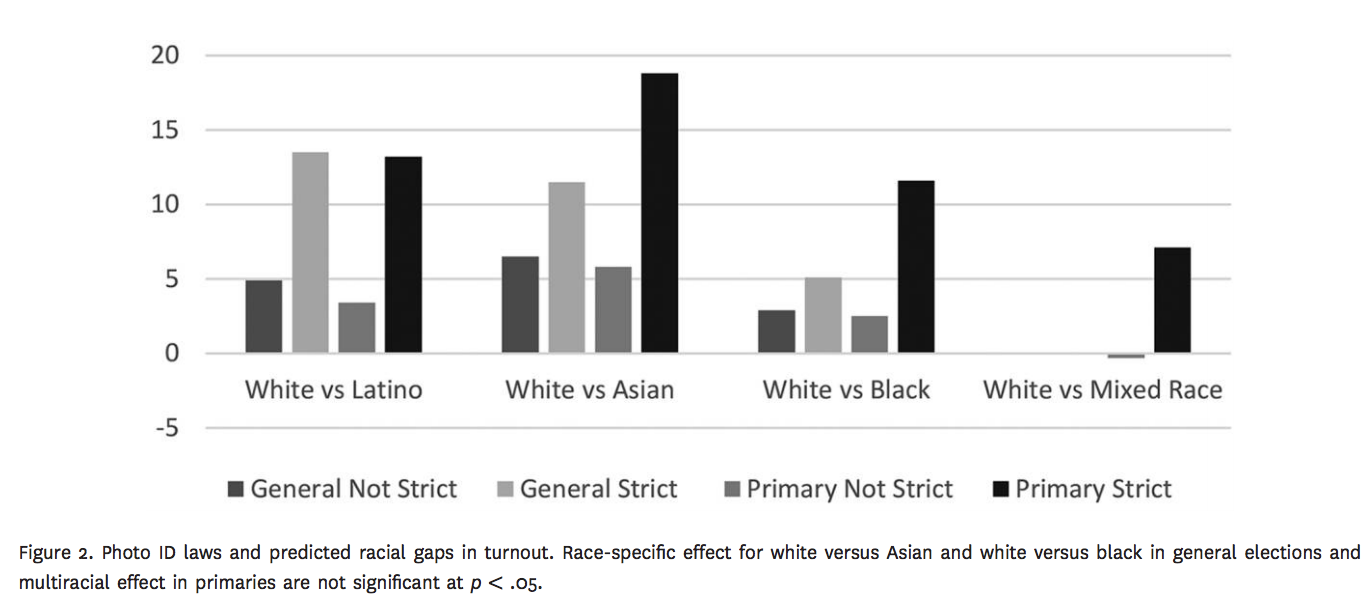
\includegraphics{JOP_Effects.png}}


\end{frame}

\begin{frame}
\frametitle{Assessing Cross Sectional Design: Placebo Test}
 \only<1-4,6>{
\begin{itemize}
	\item[-] If cross sectional (selection on observables) design works:\pause
	\begin{itemize}
	\invisible<1>{\item[-] States that implement voter ID laws are (conditionally) on average similar to states that do not} \pause 
	\invisible<1-2>{\item[-] No ``effect" of being a strict voter ID law in the past}\pause 
\end{itemize}
	\invisible<1-3>{\item[-] Placebo test: assess ``effect" of being future strict voter ID law state on turnout before law implemented} \pause 
	\invisible<1-5>{\item[-] Hajnal, Kuk, and Lejavardi (2018) suggest placebo test using difference in differences (state and year fixed effects): not possible to estimate this placebo test. 
	\begin{itemize} 
		\item[-] Why?: no within state variation on future strict voter ID law status. 
		\item[-] Coefficients from placebo test in HKL: estimated by statistical routine automatically dropping states to fit model.  Strict voter ID law reported coefficient just a state fixed effect, interaction estimated solely from within state racial composition variation
		\item[-] Does not provide an assessment of the plausibility of the design
		\end{itemize} }
\end{itemize}}

\only<5>{\scalebox{0.5}{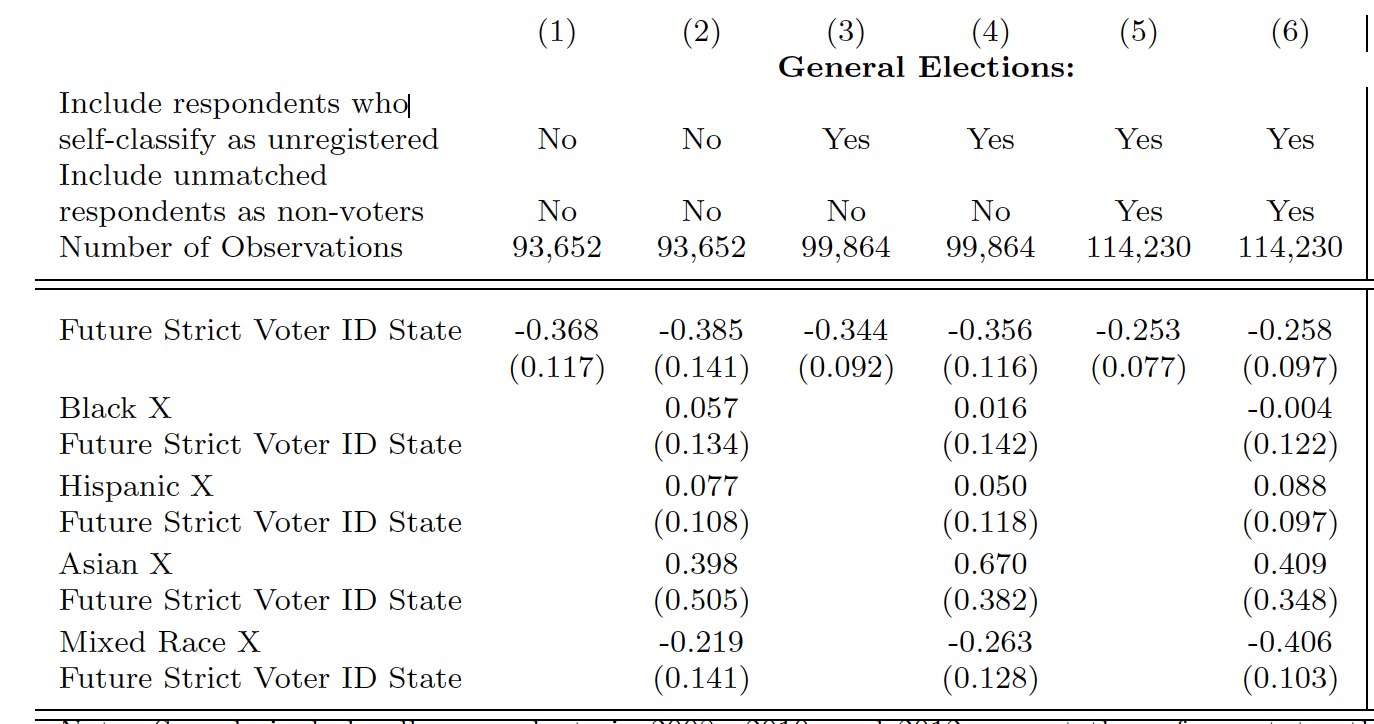
\includegraphics{Placebo.png}}}
\pause 

\end{frame}

\begin{frame}
\frametitle{Cross Sectional $\leadsto$ Difference in Differences}

\large 
Cross Sectional Design Fails $\leadsto$ Difference in Differences Design\\
HLN: ``one of the most rigorous ways to examine panel data"

\end{frame}



\begin{frame}
\frametitle{Difference in Differences Estimates, HLN}

\begin{tikzpicture}
\node (image) at (-8, 8) [] {\scalebox{0.85}{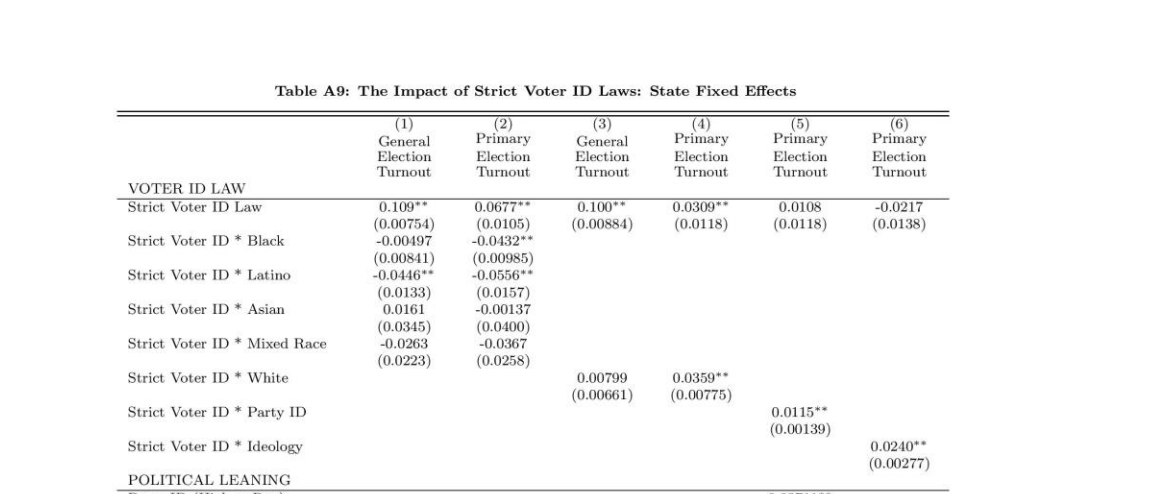
\includegraphics{DiD.png}}} ;
\node (c1) at (-15, 9) [] {} ;
\node (c2) at (-15, 8.2) [] {} ;
\node (c3) at (-10, 9) [] {} ;
\node (c4) at (-10, 8.2) [] {} ;

\node (c5) at (-15, 7.7) [] {} ;
\node (c6) at (-15, 8.2) [] {} ;
\node (c7) at (-10, 7.7) [] {} ;
\node (c8) at (-10, 8.2) [] {} ;

\node (c9) at (-15, 7.2) [] {} ;
\node (c10) at (-15, 7.7) [] {} ;
\node (c11) at (-10, 7.2) [] {} ;
\node (c12) at (-10, 7.7) [] {} ;


\only<2->{\draw[-, line width = 1.5pt] (c1) to (c2) ;
\draw[-, line width = 1.5pt] (c1) to (c3) ;
\draw[-, line width = 1.5pt] (c3) to (c4) ;
\draw[-, line width = 1.5pt] (c2) to (c4) ; }

\only<3>{\draw[-, line width = 1.5pt] (c5) to (c6) ;
\draw[-, line width = 1.5pt] (c5) to (c7) ;
\draw[-, line width = 1.5pt] (c6) to (c8) ;
\draw[-, line width = 1.5pt] (c7) to (c8) ; }


\only<4>{\draw[-, line width = 1.5pt] (c9) to (c10) ;
\draw[-, line width = 1.5pt] (c9) to (c11) ;
\draw[-, line width = 1.5pt] (c11) to (c12) ;
\draw[-, line width = 1.5pt] (c10) to (c12) ; }
\end{tikzpicture}

\end{frame}



\begin{frame}
\frametitle{Implied Effect of Voter ID Laws from Diff-in-Diff in General Elections (All Statistically Significant)}

\begin{tabular}{|ll|}
\hline \hline
		 & Estimate \\
\hline
White 			& 10.9 \\
\hline
African American &  10.4 \\
\hline
Latinos & 6.5  \\
\hline
Asian Americans & 12.5 \\
\hline
Mixed Race & 8.3 \\
\hline \hline
\end{tabular}

\end{frame}


\begin{frame}

\huge
Results are not credible $\leadsto$ due to merge error in data

\end{frame}

\begin{frame}
\Huge
\alert{WE ARE NOT ARGUING VOTER ID LAWS INCREASE TURNOUT}


\end{frame}


\begin{frame}
\frametitle{What went wrong?}

\only<1>{
CCES turnout in Virginia shows 0\% turnout in control period, plausible turnout levels in treatment period $\leadsto$ ``positive effect" due to merge error
\scalebox{0.5}{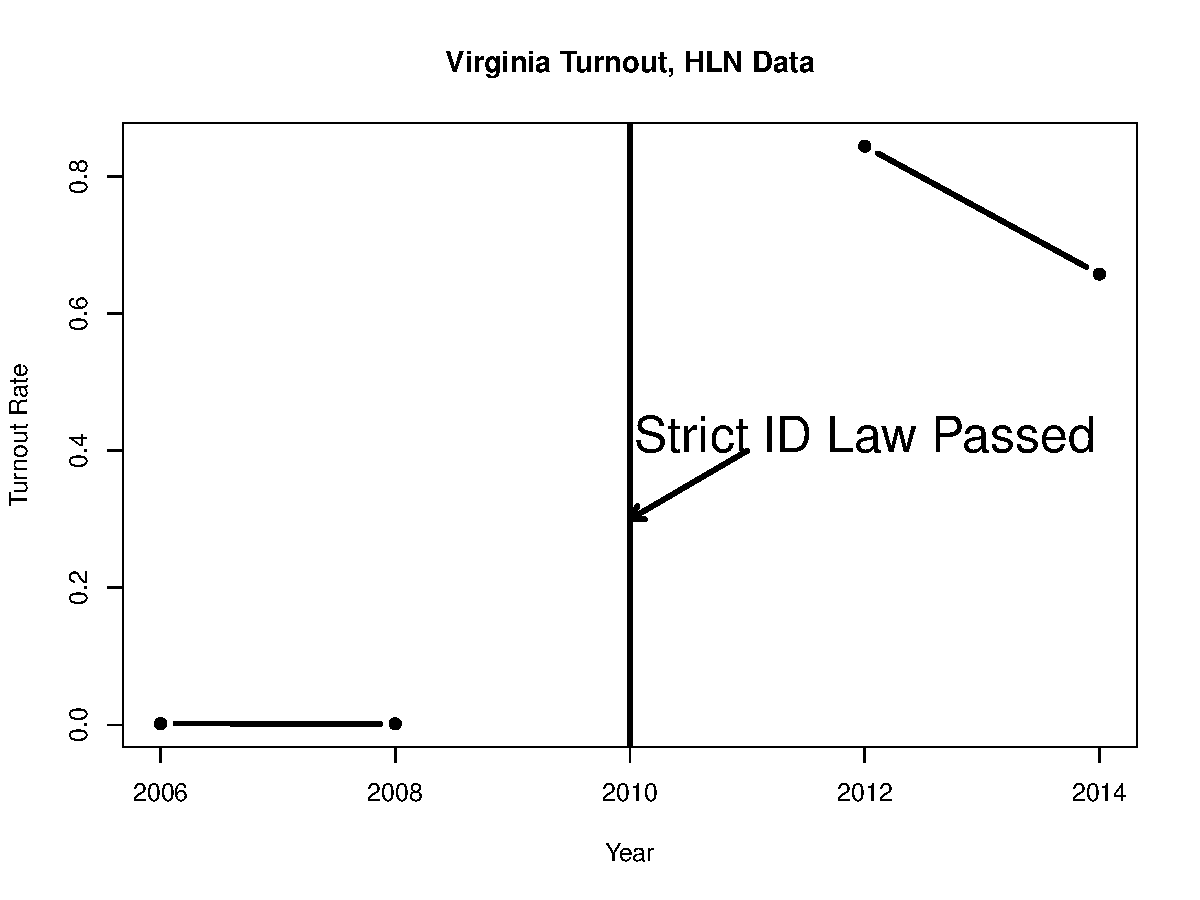
\includegraphics{VAPlot.pdf}}}
\only<2>{
To see influence of Virginia, we can drop one state at a time and assess the effect on the estimated effect of strict voter ID laws on turnout, estimated using a difference in differences design 
\scalebox{0.5}{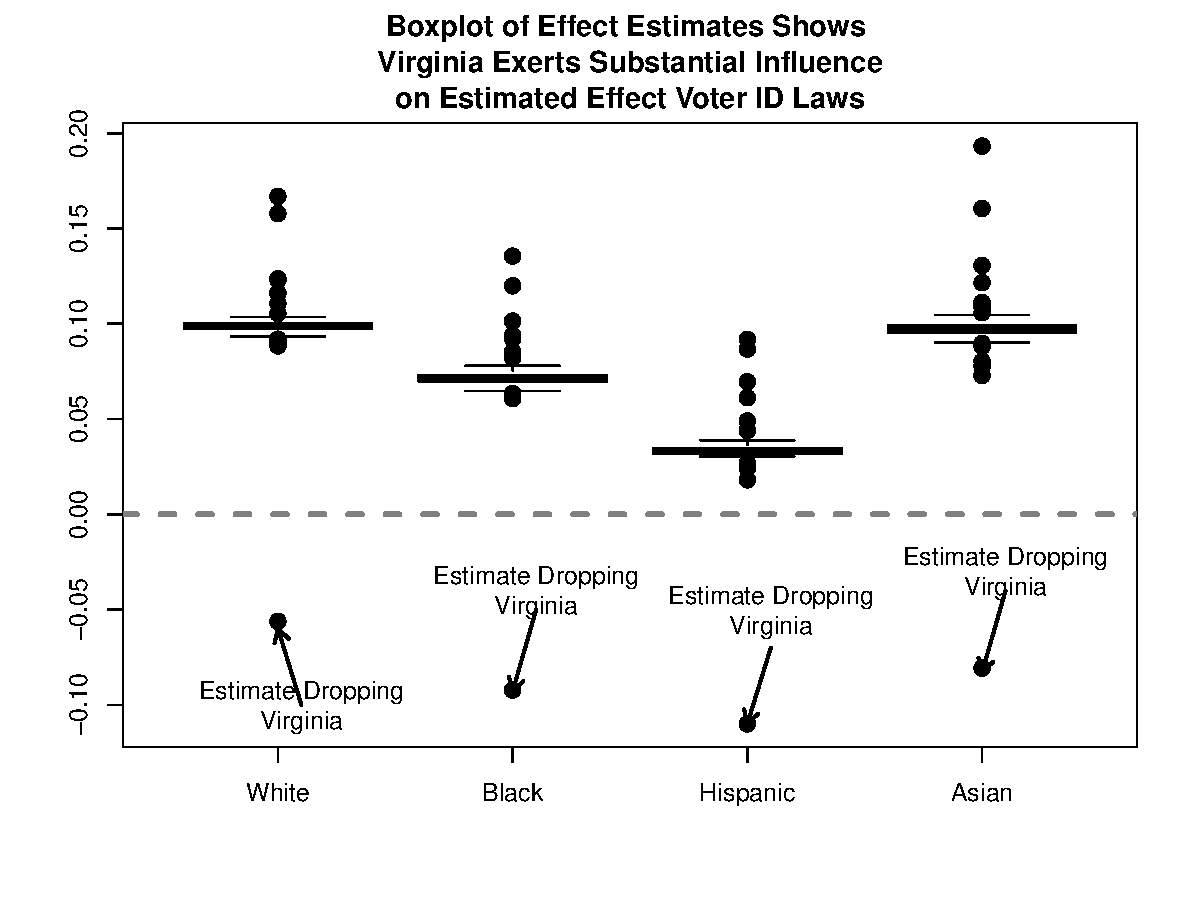
\includegraphics{DropOneStateBoxPlot.pdf}}}
\only<3>{\Large This is a risk with \alert{any} fixed effect regression

\begin{itemize}
\item[-] Use within unit variation, average across units to calculate effect
\item[-] Major Errors in one unit $\leadsto$ exercise substantial influence over estimates
\item[-] \alert{Inspect Your Data!}
\end{itemize}

}
\end{frame}

\begin{frame}
\frametitle{Other Explanations?}

\only<1>{\begin{itemize}
\item[-] \Large Hajnal, Kuk, and Lejavardi (2018): Argue specification is Missing Political Control Variables (Partisan control of governor, State House, and State Senate) 
\end{itemize}}

\only<2>{\footnotesize Originally provided political control variables had state-level missingness for states (alphabetically) from Virginia to Wyoming from 2006-2008. Figure below shows percent missing for respondents from each state for Republican governor, 2006-2008 This missingness effectively drops the problematic Virginia years from the analysis.   Once corrected, political control variables do not resolve implausible positive effects
\begin{center}
 \scalebox{0.435}{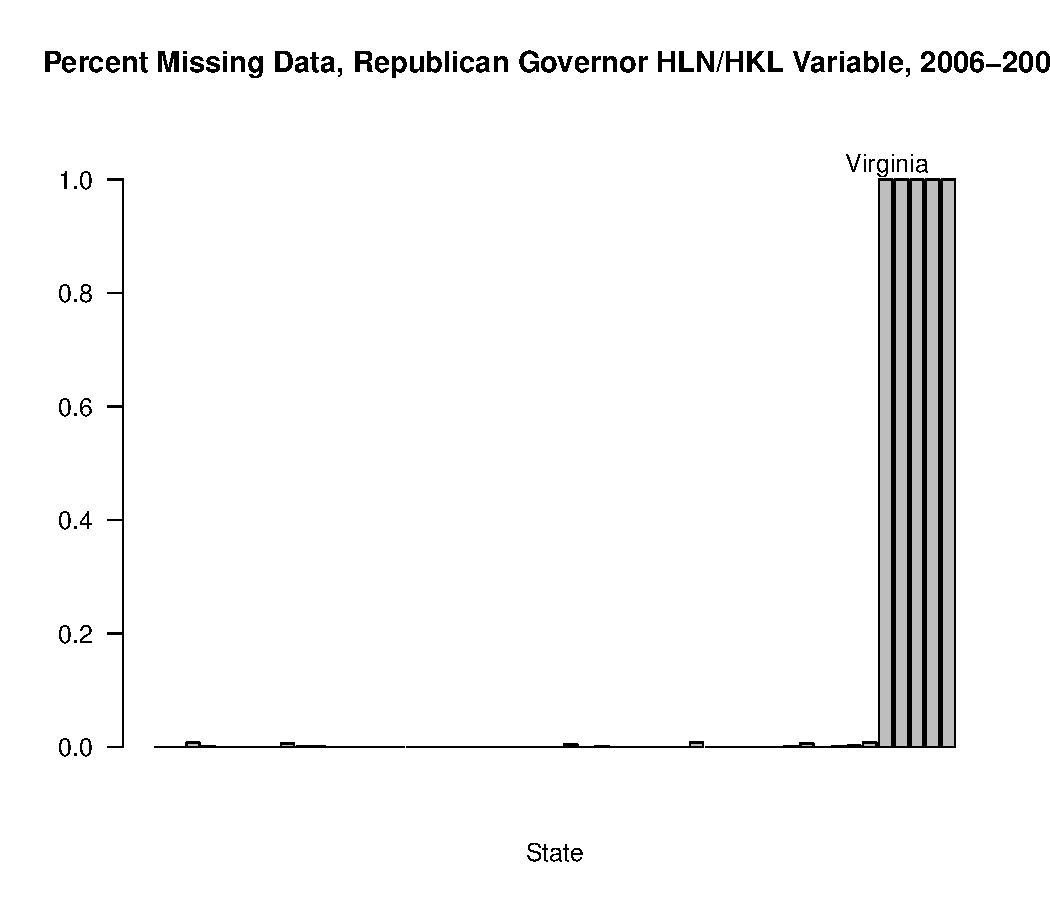
\includegraphics{MissingDataGov.pdf}}
 \end{center}
}

\only<3>{ HKL (2018) Also Argue:
	\begin{itemize}
		\item[-] No clustering of Standard Errors
		\item[-] No Survey Weights 
	\end{itemize}
}

\only<4>{\small The top estimate in each figure shows original HLN estimate of strict voter ID laws on general election turnout from difference in differences model, second is the estimate after clustering standard errors, third is estimate after including survey weights, fourth after including political controls, fifth from dropping Virginia, sixth recoding turnout so nonmatches are zero 
	\scalebox{0.6}{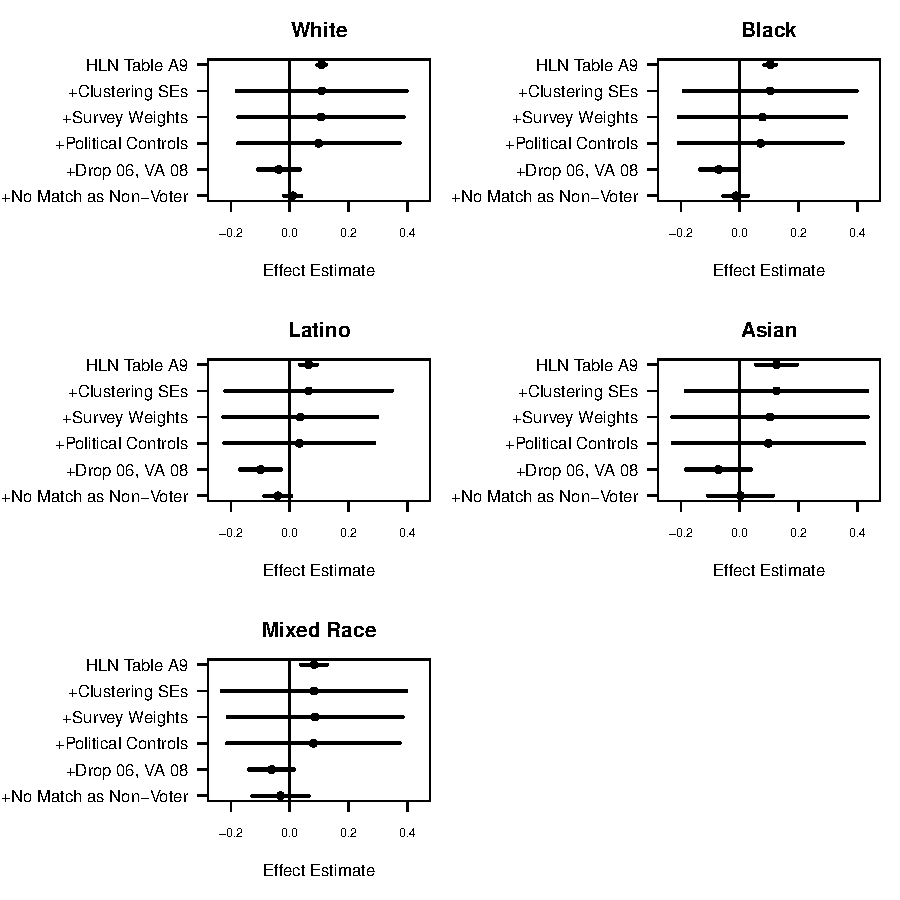
\includegraphics{rep_specs}}

}


\end{frame}


\begin{frame}
\huge
After correcting data, Survey not up to the task (Erikson and Minnite 2009) 

\end{frame}

\begin{frame}
\frametitle{Survey Data and Effects of Election Administration}

\only<1>{\scalebox{0.6}{\includegraphics{compareactualtoccesall.eps}}}
\only<2>{\scalebox{0.8}{\includegraphics{tablea9_combined.eps}}}


\end{frame}


\begin{frame}
\frametitle{How to Assess Effect of Voter ID Laws?}
\begin{itemize}
\item[-] Even with large sample CCES unable to inform debate on voter ID laws because small samples in each state
\item[-] Placebo tests: useful, but caution must be used because statistical routines drop variables to enable regression to estimate, coefficients may not reflect what you think.  
\item[-] Fixed effect regression, worry about unit-level errors that exercise substantial influence on estimates
\end{itemize}



\end{frame}



\end{document}
